% !TEX root =  ../main_iclr.tex

\begin{figure*}[t!]
\centering
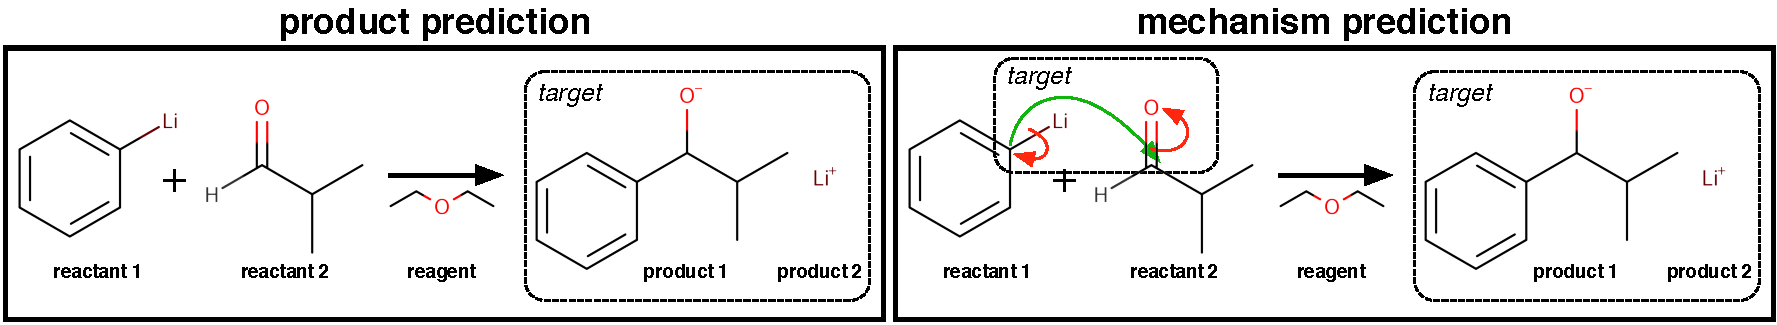
\includegraphics[width=\textwidth]{reaction_diagram.pdf}
\caption{\emph{(Left)} The reaction product prediction problem: Given the reactants and reagents, predict the structure of the product. \emph{(Right)} The reaction mechanism prediction problem: Given the reactants and reagents, predict how the reaction occurred to form the products.}
\label{fig:task-overview}

\end{figure*}

We begin with a brief background from chemistry on molecules and chemical reactions, and
then review related work in machine learning on predicting reaction outcomes. 
We then describe a particularly important subclass of chemical reactions, called \emph{linear electron flow} (LEF) reactions,
and summarize the contributions of this work.
%Finally, we summarize the contributions of this work.



\subsection{Molecules and Chemical reactions}
Organic (carbon-based) molecules can be represented via a graph structure, where each node is an atom and each edge is a covalent bond (see example molecules in Figure~\ref{fig:task-overview}).
Each edge (bond) represents two electrons that are shared between the atoms that the bond connects. 

Electrons are particularly important for describing how molecules react with other molecules to produce new ones. All chemical reactions involve the stepwise movement of electrons along the atoms in a set of reactant molecules. 
This movement causes the formation and breaking of chemical bonds that changes the reactants into a new set of product molecules \citep{herges1994coarctate}. For example, Figure~\ref{fig:task-overview} (\emph{Right}) shows how electron movement can break bonds (red arrows) and make new bonds (green arrows) to produce a new set of product molecules.

\subsection{Related work}
In general, work in machine learning on reaction prediction can be divided into two categories: (1) \emph{Product prediction}, where the goal is to predict the reaction products, given a set of reactants and reagents, shown in the left half of Figure~\ref{fig:task-overview}; and (2) \emph{Mechanism prediction}, where the goal is to determine {\em how} the reactants react, i.e., the movement of electrons, shown in the right of Figure~\ref{fig:task-overview}.


\paragraph{Product prediction.}
% wei2016neural
% NOTE: Jennifer, David and Alan were not the first to apply deep learning to this problem, this was done Aires de Sousa's group already in 2005, using unsupervised pretraining.
Recently, methods combining machine learning and template-based molecular rewriting rules have been proposed \citep{coley2017prediction,neural-symbolic,segler2018planning,wei2016neural,zhang2005structure}.
 Here, a learned model is used to predict which rewrite rule to apply to convert one molecule into another. While these models are readily interpretable, they tend be brittle. 
%The earliest work we are aware of that uses deep learning to predict the products of reactions is \cite{zhang2005structure}. Their idea was to approximate the operations of a molecular fingerprint so that all operations become continuously differentiable. They then learned parameters of this fingerprint to accurately predict product fingerprints end-to-end.
% jin2017predicting
Another approach, introduced by \cite{jin2017predicting}, constructs a neural network based on the Weisfeiler-Lehman algorithm for testing graph isomorphism. They use this algorithm (called WLDN) to select atoms that will be involved in a reaction. They then enumerate all chemically-valid bond changes involving these atoms and learn a separate network to rank the resulting potential products. This method while leveraging new techniques for deep learning on graphs, cannot be trained end-to-end because of the enumeration steps which ensures chemical validity.
% schwaller2017found
\cite{schwaller2017found} represents reactants as SMILES \citep{weininger1988smiles} strings and then uses a sequence to sequence network (specifically, the work of \citet{Zhao2017}) to predict product SMILES. While this method (called Seq2Seq) is end-to-end trainable, the SMILES representation is quite brittle as often single character changes will not correspond to a valid molecule.

 These latter two methods, WLDN and Seq2Seq, are state-of-the-art on product prediction and have been shown to outperform the above template-based techniques \citep{jin2017predicting}. Thus we compare directly with these two methods in this work.

% segler2017modelling
% TODO
% segler2018planning
% TODO

\paragraph{Mechanism prediction.}
The only other works we are aware of to use machine learning to predict reaction mechanisms are \citet{fooshee2018deep,NIPS2011_4356,kayala2012reactionpredictor,kayala2011learning}. All of these model a chemical reaction as an interaction between atoms as electron donors and as electron acceptors. They predict the reaction mechanisms via two independent models: one that identifies these likely electron sources and sinks, and another that ranks all combinations of them.
These methods have been run on small expert-curated private datasets, which contain information about the reaction conditions such as the temperature and anion/action solvation potential \citep[\S2]{NIPS2011_4356}.
In contrast, in this work, we aim to learn reactions from noisy large-scale public reaction datasets, which are missing the required reaction condition information required by these previous works.
As we cannot yet apply the above methods on the datasets we use, nor test our models on the datasets they use, as they are not yet publicly released, we cannot compare directly against them; therefore, we leave a detailed discussion of the pros and cons of each method for future work.

%we leave a detailed comparison of the pros and cons of both methods for future work.
 % (unfortunately the data used to train these models is not currently open-source). 
%However, 
%this combining and then ranking of electron sources and sinks can be a slow process, as many plausible reactions need to be considered \emph{for each electron movement} (the number of subgraphs of $n$ reacting atoms, where single bonds are either added or removed is $2^{n(n-1)/2}$). Furthermore, 
%these models rely on expert-curated training sets, for which organic chemists have to hand-code every electron pushing step (unfortunately the data used to train these models is not currently open-source). As such, this work is complimentary to ours
%These models also have only so far been successfully trained on small hand-curated datasets.
% kayala NIPS: NIPS2011_4356
% kayala2011learning
% kayala2012reactionpredictor
% fooshee2018deep

As a whole, this related work points to at least two main desirable characteristics for reaction prediction models: 
\begin{enumerate}
\item \emph{End-to-End}: There are many complex chemical constraints that limit the space of all possible reactions. How can we differentiate through a model subject to these constraints?
%\item \emph{Graph-Based}: Recent successes in deep learning models for graphs can embed similar graphs to similar vectors. How can we use such models to predict graphs?
\item \emph{Mechanistic}: Learning the mechanism offers a number of benefits over learning the products directly including: interpretability (if the reaction failed, what electron step went wrong), sparsity (electron steps only involve a handful of atoms), and generalization (unseen reactions also follow a set of electron steps).
\end{enumerate}

%In general, a model that predicts the reaction mechanism has a number of benefits over predicting the product of reaction directly: (a) \textbf{interpretability}: If the model makes a mistake, it is easy to see where, and possibly why, it goes wrong by comparing the steps of the mechanism with the correct steps. (b) \textbf{sparse}: Reactions often only affect between 3 and 7 atoms out of anywhere from 10-50 reactant atoms. Modeling the reaction as a path allows one to exploit this sparsity. (c) \textbf{chemically constrained}: Learning a path allows one to easily incorporate chemical constraints, such as the alternating removal and addition of bonds, among others. (d) \textbf{generalizable}: As reaction paths follow similar trends in different molecules, mechanistic models naturally generalize to unseen molecules. 



% We argue that there are a number of benefits of predicting electron paths over predicting the outcomes of reactions directly (as is done in previous work \cite{jin2017predicting,schwaller2017found}):
% \begin{itemize}
% \item \textbf{Easy to interpret}: If the model makes a mistake, it is easy to see where, and possibly why, it goes wrong by comparing the steps of the path with the correct steps.
% \item \textbf{Sparse}: Reactions often only affect between 3 and 7 atoms out of anywhere from 10-50 reactant atoms. Modeling the reaction as a path allows us to exploit this sparsity.
% \item \textbf{Chemically consistent}: Learning a path allows us to easily incorporate chemical constraints, such as the alternating removal and addition of bonds, among others. 
% \item \textbf{Generalizable}: As reaction paths follow similar trends in different molecules, our model naturally generalizes to unseen molecules. 
% \end{itemize}

 



%\begin{wrapfigure}{R}{0.75\textwidth}
%\scriptsize{
%\vspace{-4ex}
%\begin{minipage}{0.75\textwidth}
\begin{table*}[t]
\begin{tabular}{lccc} 
\toprule
 \textbf{Prior Work} & \textbf{end-to-end}  & \textbf{mechanistic} &  \\ %\hline \hline
\midrule
Templates+ML & $-$  & $-$   \\ 
%\cite{coley2017prediction} & $-$ & $-$ & $-$ \\ \hline
WLDN [\cite{jin2017predicting}] &$-$ & $-$  \\ 
Seq2Seq [\cite{schwaller2017found}] & \checkmark & $-$  \\ 
%\cite{segler2017modelling} & \checkmark & $-$ & $-$ \\ \hline 
%\cite{segler2018planning} & \checkmark & \checkmark & $-$  \\ \hline
%\cite{NIPS2011_4356} &$-$ & $-$ & \checkmark  \\ \hline
%\cite{kayala2011learning} & $-$ & $-$ & \checkmark \\ \hline
%\cite{kayala2012reactionpredictor} &$-$ & $-$ &\checkmark  \\ \hline
Source/Sink (expert-curated data) & $-$ & \checkmark \\ 
\midrule
\textbf{This work} & \checkmark  & \checkmark \\
\bottomrule
%\bf{Method} & %\multicolumn{2}{c}{\bf Full} & \multicolumn{2}{c}{\bf Unaware} & \multicolumn{2}{c}{\bf Fair L2} & \multicolumn{2}{c}{\bf Fair L3} \\
\end{tabular}
\centering
	\caption{Work on machine learning for reaction prediction, and whether they are (a) end-to-end trainable, and (b) predict the reaction mechanism. \label{table.existing}}
\end{table*}
%\end{minipage}
%\vspace{-4ex}
%}
%\end{wrapfigure}


Table~\ref{table.existing} describes how the current work on reaction prediction satisfies these characteristics. In this work we propose to model a subset of mechanisms with \emph{linear electron flow}, described below.

\subsection{Linear Electron Flow reactions} \label{sect:LEF}
%


Reaction mechanisms can be classified by the topology of their ``electron-pushing arrows'' (the red and green arrows in Figure~\ref{fig:task-overview}). 
Here, the class of reactions with \emph{linear electron flow} (LEF) topology is by far the most common and fundamental, followed by those with cyclic topology \citep{herges1994coarctate}. 
In this work, we will only consider LEF reactions that are \emph{heterolytic}, i.e., they involve pairs of electrons.\footnote{The treatment of radical reactions, which involve the movement of single electrons, will be the topic of future work.}

If reactions fall into this class, then a chemical reaction can be modelled as pairs of electrons moving in a \emph{single path} through the reactant atoms. 
In arrow pushing diagrams representing LEF reactions, this electron path can be represented by arrows that line up in sequence, differing from for example pericyclic reactions in which the arrows would form a loop \citep{herges1994coarctate}.


Further for LEF reactions, the movement of the electrons along the linear path will alternately remove existing bonds and form new ones. 
We show this alternating structure in the right of Figure \ref{fig:task-overview}. 
The reaction formally starts by (step 1) taking the pair of electrons between the Li and C atoms and moving them to the C atom; this is a remove bond step. 
Next (step 2) a bond is added when electrons are moved from the C atom in reactant 1 to a C atom in reactant 2.
Then (step 3) a pair of electrons are removed between the C and O atoms and moved to the O atom, giving rise to the products. 
Predicting the final product is thus a byproduct of predicting this series of electron steps.


\paragraph{Contributions.} We propose a novel generative model for modeling the reaction mechanism of LEF reactions. Our contributions are as follows:
\begin{itemize}
\item We propose an end-to-end generative model for predicting reaction mechanisms, \ourModelR, that is fully differentiable. It can be used with any deep model on graphs.
\item We design a technique to identify LEF reactions and mechanisms from purely atom-mapped reactants and products, the primary format of large-scale reaction sets.
\item We show that \ourModelR learns chemical knowledge such as functional group selectivity without explicit training.
\end{itemize}


